\documentclass{beamer}
\usepackage{beamerthemeCambridgeUS}
\usepackage{color}  % for \textcolor{red}{blah}
\usepackage{graphicx}
\usepackage{subfigure}
\usepackage{multicol}
\usepackage{verbatim} % for \begin{comment}
\usepackage{lipsum}


\newcommand\Fontvi{\fontsize{6}{7.2}\selectfont}


\newenvironment{packed_enum}{
\begin{enumerate}
  \setlength{\itemsep}{1pt}
  \setlength{\parskip}{0pt}
  \setlength{\parsep}{0pt}
}{\end{enumerate}}

\newenvironment{packed_item}{
\begin{itemize}
  \setlength{\itemsep}{1pt}
  \setlength{\parskip}{0pt}
  \setlength{\parsep}{0pt}
}{\end{itemize}}

\usetheme{CambridgeUS}

\title{Discrete Mathematics}
\author[Geoffrey Buhl]{Geoffrey Buhl \\ \texttt{geoffrey.buhl@csuci.edu}}
\institute[CSUCI]{California State University Channel Islands}
\date{week 5 class 1}

\def \vec{{\rm vec}}
\newtheorem{conjecture}[theorem]{Conjecture}
\newtheorem{explanation}[theorem]{Explanation}


\begin{document}

%\frame{\titlepage}

%\section[Outline]{}
%\frame{\tableofcontents}

\section{Week 5 Class 1}

\frame
{
  \frametitle{Introduction to Recursion}

Chapter 2 covers using recursion to count objects.  Two important questions to ask are:  If I know the answer for the $n$ case, what do I need to do to get the answer to the $n+1$ case?  Can I find a smaller versions of the problem in the problem I am working on?
\vfill
Class Session Goals:
\begin{packed_enum}
\item Present recursion in the mathematical context
\item Practice creating recursive formulas for sequences
\end{packed_enum}
\vfill
}

\frame
{
  \frametitle{Interesting Mathematical Sequences}


\begin{tabular}{lll}
Sequence & Name & OEIS\\ \hline
$1,2,3,4,5,6, \ldots$ &Counting & A000027 \\
$1,3,6,10,15,21, \ldots$ &Triangular & A000217\\
$1,4,9,16,25,36, \ldots$ &Square &A000290 \\
$1,1,2,3,5,8, \ldots$ &Fibbonacci &A000045 \\
$0, 2, 5, 9, 14, 20, \ldots$ &???&A000096\\
\end{tabular}
\vfill
Sequences give the answer to questions like: What is the sum of the first $n$ integers?  What is the sum of the first $n$ odd integers? How many diagonals are there in a $n+2$-gon?

}


\frame
{
  \frametitle{Recursive and Closed Formula}

We can express sequences recursively or in a closed form.  Closed form means as a function of $n$.\vfill

\begin{tabular}{llll}
Numbers & Initial Condition & Recursive Relationship & Closed Form \\ \hline
Counting & $c_1=1$ & $c_n=c_{n-1}+1$ & $c_n=n$\\
Triangular & $T_1=1$ & $T_n=T_{n-1}+n$ & $T_n=\frac{n(n+1)}{2}$\\
Square& $S_1=1$ & $S_n=S_{n-1}+2n-1$ & $S_n=n^2$\\
Fibbonacci& $F_1=1,F_2=1$ & $F_n=F_{n-1}+F_{n-2}$ & $T_n=???$\\
$n+2$-gon Diags& $D_1=0$ & $D_n=???$ & $D_n=\frac{n(n+3)}{2}$
\end{tabular}
\vfill
%Other examples:  Diagonal for an $n$-gon

}

\frame
{
  \frametitle{A few definitions}

The {\bf order} of a recursive formula is the number of preceding values that are needed to calculate the next value.  For example, the Fibonnacci recursion has order 2, and the Triangular number recursion has order 1.\vfill

A recurrence is called {\bf linear} if it has the form $$a_n=c_1\cdot a_{n-1}+c_2\cdot a_{n-2} \cdots + c_k\cdot a_{n-k} +f(n)$$ where $c_i$ are real numbers and $f(n)$ is a function of $n$.  If $f(n)=0$ the recurrence is called {\bf homogeneous} and if $f(n) \ne0$ the recurrence is called {\bf non-homogeneous}. All the examples on the previous slide are linear, but the Fibbonacci sequence is the only homogenous linear example on the last slide.\vfill

If a recurrence is not linear, the it is called a {\bf non-linear} recurrence relation. An example of a non-linear recurrence is $a_n=a_{n-1}\cdot a_{n-3}$.\vfill


}


\frame
{
  \frametitle{Goal for the next two classes}

The most challenging part of chapter 2 is going from a counting problem to a recursive representation of the problems.  We will explore two ways to do this motivated the following two questions.\vfill


\begin{packed_enum}
\item Can I find patterns in the differences in small $n$ data?
\item Can I find smaller versions of my problem?
\end{packed_enum}


}

\frame
{
  \frametitle{Recursion Activity}

For the remainder of the next  two classes, we will work on a number of counting problems where the goal is to find a recursive formula that gives the answers to the following counting problems.  In the next few classes we will learn how to calculate a closed form solution if we have a recursive description of the solution.
\vfill

\begin{packed_enum}
\item $F_n$ - number of different $n$ strip flags
\item $V_n$ - area of the $n$th Von Neumann neighborhood
\item $P_n$ -  $n$th Pentagonal number
\item $C_n$ - maximum pieces of cake with $n$ cuts
\item $H_n$ - minimum moves needed to solve a Tower of Hanoi problem with 
\item $T_n$ - tilings of a $1\times n$ board by $1 \times 2$ and $1 \times 1$ tiles
\item $S_n$ - different ascents of an $n$-stair staircase
\item $B_n$ - binary strings of length $n$ that include 00
\end{packed_enum}

}


\frame
{
  \frametitle{Flags}

Suppose you have 3 colors, and you are creating a flag with $n$ horizontal stripes with the condition that adjacent stripes must be different colors.  Let $F_n$ be the number of ways to create an $n$ stripe flag. Can you express $F_n$ as a recursion? Can you find a closed form?\vfill
Some examples of a 3 stripe flag.
  \begin{figure}[htp]
  \begin{center}
    \subfigure{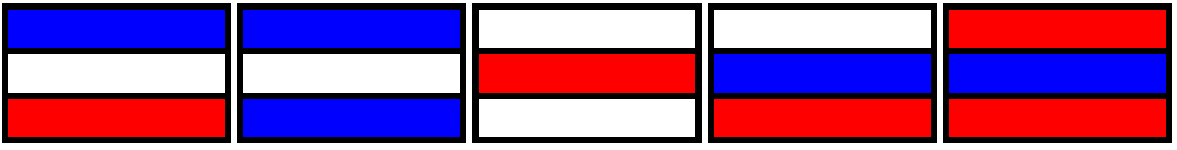
\includegraphics[scale=.45]{flags}}
    \end{center}
\end{figure}
%What if the flag must have a different color on the top and bottom?
}

\frame
{
  \frametitle{Von Neumann Neighborhoods}

  What is the size of the $n$th Von Neumann Neighborhood?  Let $V_n$ be the number of squares in the $n$th Von Neumann Neighborhood. Can you find a recursive formulas for $V_n$?  Can you find a closed form? 
  \begin{figure}[htp]
  \begin{center}
    \subfigure{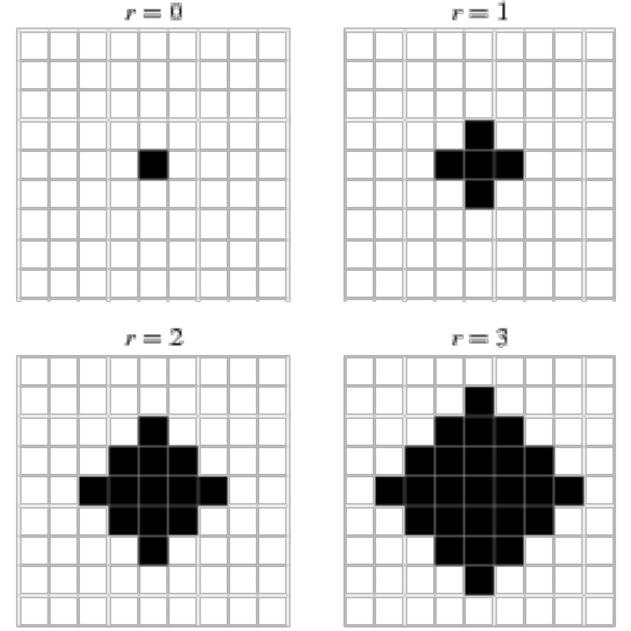
\includegraphics[scale=.5]{vonNeumannNeighborhood_800}}
    \end{center}
\end{figure}
 %What about the 3-dimensional analogue?
%\pause $V_n=V_{n-1}+n$
}

\frame
{
  \frametitle{Pentagonal Numbers}
 How many dots are in the $n$th pentagonal diagram?  Let $P_n$ be the number of dots  in the $n$th pentagonal diagram. Can you find a recursive formulas for $P_n$?  Can you find a closed form?

\begin{figure}[htp]
  \begin{center}
    \subfigure{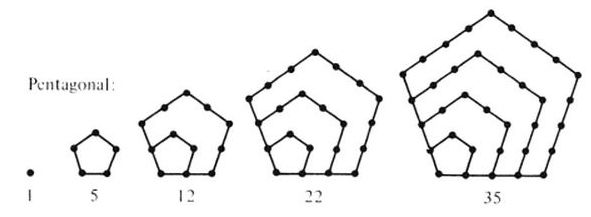
\includegraphics[scale=.50]{pentagonal}}
  \end{center}
\end{figure}

$P_1=1$, $P_2=5$, $P_3=12$, $P_4=22$, $P_5=35$
}

\frame
{
  \frametitle{Lazy Caterer}

What is the maximum number of pieces you can cut a circular cake into with $n$ cuts, call this $C_n$?  Can you express $C_n$ as a recursion? Can you find a closed form? \vfill
Pictures for $n=0,1,2$.
  \begin{figure}[htp]
  \begin{center}
    \subfigure{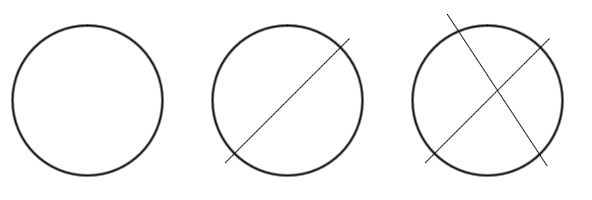
\includegraphics[scale=.45]{caterer2}}
    \end{center}
\end{figure}
%What if it's a spherical cake and cuts can be in any plane?
}


\frame
{
  \frametitle{Towers of Hanoi}

 What is the smallest number of moves to solve the Towers of Hanoi puzzle with $n$ disks.?  Let $H_n$ be the minimun moves in an $n$-disk solution. What are some initial values? Can you find a recursive formulas for $H_n$?  Can you find a closed form?  \begin{figure}[htp]
  \begin{center}
    \subfigure{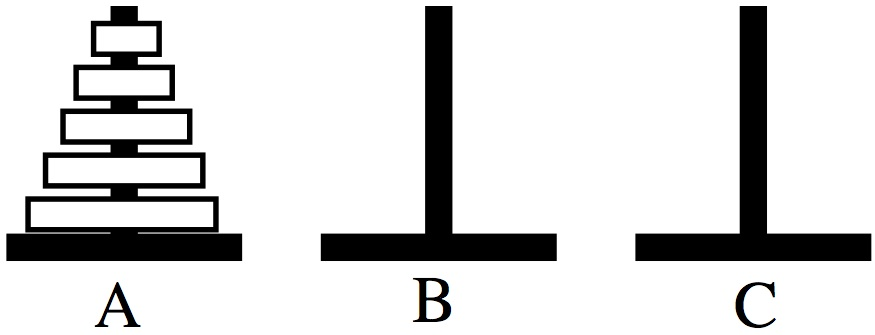
\includegraphics[scale=.25]{TowersOfHanoiFigure}}
    \end{center}
\end{figure}
%What if can only move to an adjacent post? What if there is a 4th post?
%\pause $T_n=2T_{n-1}+1$, $T_n=2^n-1$
}


\frame
{
  \frametitle{Tiling a sidewalk}

 How many ways can you tile a $1 \times n$ board with a $1 \times 1$ squares and $2 \times 1$ rectangles, call this $T_n$?  Can you express $T_n$ as a recursion? Can you find a closed form?\vfill
 Here are five possible tilings of a $1 \times 4$ board.
  \begin{figure}[htp]
  \begin{center}
    \subfigure{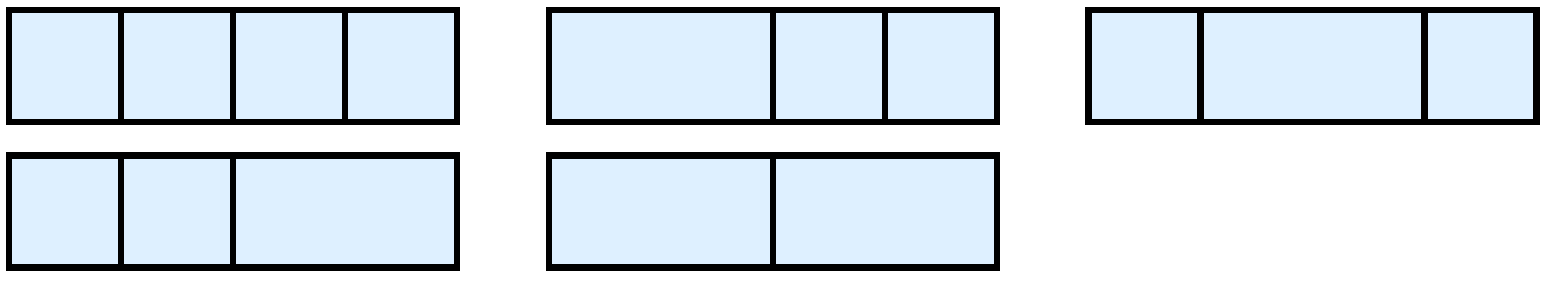
\includegraphics[scale=.40]{FibonacciTiling4}}
    \end{center}
\end{figure}
%What if you have two different types of $1 \times 1$ squares, say white and black?
%\pause $T_1=1$, $T_2=2$, $T_n=T_{n-1}+T_{n-1}$
}






\frame
{
  \frametitle{Staircase Problem}

How many ways can you walk up a staircase with $n$ stairs if you can choose 1, 2, or 3 steps to ascent?  Let $S_n$ be the number of different ascents of a $n$-step staircase. Can you express $S_n$ as a recursion? Can you find a closed form? \vfill
Three different ascents of a 4 stair staircase.
  \begin{figure}[htp]
  \begin{center}
    \subfigure{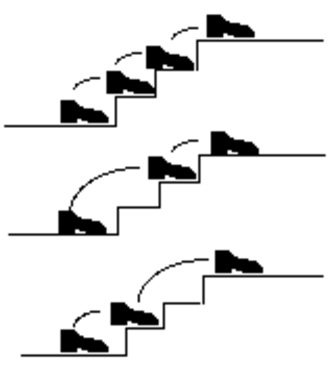
\includegraphics[scale=.50]{stairs}}
    \end{center}
\end{figure}
%What if you can choose 1, 2, 3, or 4 steps to ascend?
}





\frame
{
  \frametitle{Binary Stings}

How many binary strings of length $n$ are there that include a 00, i.e two adjacent zeros? Can you express $S_n$ as a recursion? Can you find a closed form? \vfill

}



\end{document}

